\chapter{フェルミオン、ディラック行列、ディラックの海}

ディラックの海が我々の目的地であるが、そこへの道筋が重要である。相対論的電子論における負エネルギーに直面する前に、二つの道具立てが必要である。まず、フェルミオンをボソンから区別する演算子代数が来る。次に、一次元ディラック方程式の復習が来る。そこでは、波動関数のあらゆる拡大が、三次元空間の幾何学なしに見て取れる。これらの道具立てが揃えば、三次元方程式が自らの行列構造を強いることになり、充填されたフェルミオン状態と空のフェルミオン状態についての冒頭の議論が、陽電子への鍵として戻ってくる。

我々は\(c=\hbar=1\)を用いる。大文字の\(P\)は運動量演算子を表し、小文字の\(p\)は運動量固有値を表し、太字の記号はそれらの三次元版を表す。

\section{交換は演算子代数となる}

二つの同種粒子を考え、一方が\(x\)に、他方が\(y\)にあるとする。ラベル\(x\)と\(y\)は完全な位置を表し、単一粒子の二つのデカルト座標ではない。二つの生成演算子を真空に作用させると
\begin{equation}
\lvert x,y\rangle
=
\psi^\dagger(x)\psi^\dagger(y)\lvert0\rangle.
\label{eq:l10-two-particle-state}
\end{equation}

ボソンでは、二つのスロットを交換しても状態は変わらない：
\begin{equation}
\lvert x,y\rangle=\lvert y,x\rangle.
\end{equation}
この対称性を保証する演算子の関係式は
\begin{equation}
\psi^\dagger(x)\psi^\dagger(y)
=
\psi^\dagger(y)\psi^\dagger(x).
\label{eq:l10-boson-exchange}
\end{equation}
である。二つのボソン的生成演算子は可換であるから、それらが生成する状態を変えることなく順序を逆にできる。

フェルミオンでは、交換は符号を変える：
\begin{equation}
\lvert x,y\rangle=-\lvert y,x\rangle.
\label{eq:l10-fermion-state-exchange}
\end{equation}
孤立した状態ベクトルの全体的な符号は観測可能ではないが、選択肢間の相対的な符号は観測可能であるから、このマイナス符号は一貫して運ばなければならない。式~\eqref{eq:l10-fermion-state-exchange}は
\begin{equation}
\psi^\dagger(x)\psi^\dagger(y)
=
-\,\psi^\dagger(y)\psi^\dagger(x).
\label{eq:l10-fermion-operator-exchange}
\end{equation}
を要求する。

\begin{figure}[htbp]
\centering
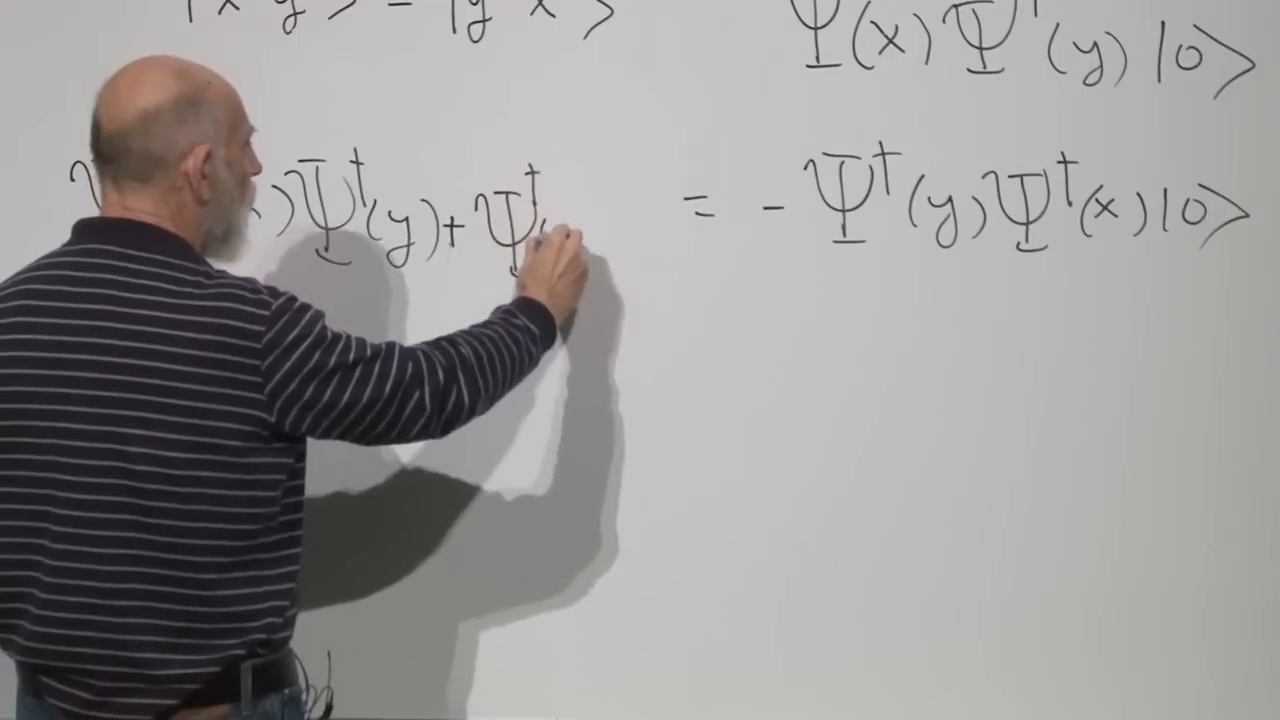
\includegraphics[width=0.94\linewidth]{lecture_10_figure_02.png}
\caption{フェルミオン的交換を実装する黒板上の関係式。生成演算子を入れ替えると二粒子状態の符号が反転する。}
\lectureframe{00:05:50}
\end{figure}

任意の二つの演算子\(A\)と\(B\)に対し、反交換子を
\begin{equation}
\{A,B\}:=AB+BA.
\end{equation}
で定義する。したがって交換規則は
\begin{equation}
\{\psi^\dagger(x),\psi^\dagger(y)\}=0.
\label{eq:l10-creation-anticommutator}
\end{equation}
である。対応するフェルミオン的場の代数は、ボソン的交换子を反交換子に置き換える。この語の二つの用法を区別して保たなければならない：場の演算子はフェルミ統計のために反交換し、一方、行列は後に相対論的分散関係における交差項を相殺するために反交換することになる。

ここで式~\eqref{eq:l10-creation-anticommutator}において\(y=x\)と置く。二つの積は同じものになる。
\begin{align}
0
&=\{\psi^\dagger(x),\psi^\dagger(x)\}\\
&=2\,\psi^\dagger(x)\psi^\dagger(x).
\end{align}
したがって
\begin{equation}
\bigl(\psi^\dagger(x)\bigr)^2=0.
\label{eq:l10-exclusion}
\end{equation}
同じ一粒子状態に二つの同種のフェルミオンを生成しようとすると、零ベクトルが得られる。これが演算子で表した排他原理である。

\begin{figure}[htbp]
\centering
\includegraphics[width=0.94\linewidth]{lecture_10_figure_03.png}
\caption{黒板上での等状態への特殊化。繰り返された生成演算子の積が二度現れるため、消えなければならない。}
\lectureframe{00:08:04}
\end{figure}

\begin{figure}[htbp]
\centering
\begin{adjustbox}{max width=\linewidth}
\begin{tikzpicture}[node distance=1.25cm,>=Latex]
\node[draw,rounded corners,align=center,inner sep=7pt] (a)
  {$\{\psi^\dagger(x),\psi^\dagger(x)\}=0$};
\node[draw,rounded corners,align=center,inner sep=7pt,right=of a] (b)
  {$2(\psi^\dagger(x))^2=0$};
\node[draw,rounded corners,align=center,inner sep=7pt,right=of b] (c)
  {$(\psi^\dagger(x))^2=0$};
\draw[->,thick] (a) -- (b);
\draw[->,thick] (b) -- (c);
\end{tikzpicture}
\end{adjustbox}
\caption{部分的に消された中間の黒板の作業なしに再構成された排他の議論。}
\end{figure}

\section{なぜフェルミオンでは充填と空が対称なのか}

ボソン的演算子とフェルミオン的演算子の間には、排他よりも微妙で、後に本質的となる第二の違いがある。単一のボソンモードに対して、
\begin{equation}
[a,a^\dagger]=1,
\qquad
n=0,1,2,\ldots.
\end{equation}
\(a\)と\(a^\dagger\)を入れ替えると交換子の符号が変わる。たとえ演算子が単に\(A\)と\(B\)と呼ばれていたとしても、代数はどちらの順序が占有数を上げ、どちらが下げるかを教えてくれる。

ボソン的占有はしごにも向きがある。消滅演算子はやがて\(\lvert0\rangle\)に達して零を与えるが、生成演算子は無限に続くことができる：
\begin{align}
a\lvert0\rangle&=0,\\
a^\dagger\lvert n\rangle&\propto\lvert n+1\rangle,
\qquad n=0,1,2,\ldots.
\end{align}
このはしごを上下逆にしても同じスペクトルは再現されない。底はあるが頂上はない。

単一のフェルミオンモードに対して、
\begin{equation}
\{a,a^\dagger\}=1,
\qquad
a^2=(a^\dagger)^2=0,
\qquad
n=0,1.
\label{eq:l10-fermion-mode}
\end{equation}
生成演算子は空の状態を充填された状態へと移し、そこで止まる：
\begin{equation}
a^\dagger\lvert0\rangle=\lvert1\rangle,
\qquad
a^\dagger\lvert1\rangle=0.
\end{equation}
消滅演算子は逆を行う：
\begin{equation}
a\lvert1\rangle=\lvert0\rangle,
\qquad
a\lvert0\rangle=0.
\end{equation}
状態は二つしかないので、図は充填と空、および\(a\)と\(a^\dagger\)の交換の下で対称である。演算子は依然として異なる物理的意味を持つが、その代数はもはや一方を生成、他方を消滅として選び出さない。この形式的対称性が粒子-正孔再解釈の種である。

\begin{classroomqa}
\lecturetimestamp{00:13:54}
\audiencequestion{もし\((a^\dagger)^2=0\)ならば、それは矛盾なのか、それとも\(a^\dagger=0\)を意味するのか？}
\lecturerresponse{どちらでもない。非零の演算子は零の二乗を持ちうる。ここで\(a^\dagger\)は\(\lvert0\rangle\)を\(\lvert1\rangle\)へと移すが、\(\lvert1\rangle\)の上には許された状態が存在しないので、二度作用させると零を与える。同じ推論により\(a^2=0\)が得られる。}
\end{classroomqa}

この「埋まった状態と空の状態」の対称性は、取っておこう。負エネルギーの電子が取り除かれると、消滅演算子は陽電子の生成演算子として読み替えられる。この移行は恣意的な記法の変更ではなく、ここで確立した二状態フェルミオン代数をまさに用いるものである。

\section{一次元ディラック構成}

ここで、一次元空間中の一粒子に戻ろう。最も単純な一階の相対論的波動方程式は
\begin{equation}
i\partial_t\psi=-\,i\partial_x\psi.
\label{eq:l10-right-mover}
\end{equation}
であり、\(P=-i\partial_x\)を用いれば
\begin{equation}
H=P.
\end{equation}
となる。運動量固有状態は\(E=p\)を持ち、その群速度は
\begin{equation}
v_g=\frac{dE}{dp}=1.
\end{equation}
である。正または負の運動量、したがって正または負のエネルギーは、依然として剛体的に右へ進む波を与える。\(p\)の符号は位相パターンを変えるのであって、伝播方向を変えるのではない。

質量を持つ粒子はどちらの方向にも動けなければならない。
\begin{equation}
H\psi_1=P\psi_1,
\qquad
H\psi_2=-P\psi_2.
\label{eq:l10-two-directions}
\end{equation}
を満たす第二の成分を導入しよう。第一の成分は右へ動き、第二の成分は左へ動く。それらを列にまとめ、
\begin{equation}
\Psi=
\begin{pmatrix}
\psi_1\\
\psi_2
\end{pmatrix},
\end{equation}
とし、
\begin{equation}
\alpha=
\begin{pmatrix}
1&0\\
0&-1
\end{pmatrix}.
\end{equation}
を定義する。両方の方程式は
\begin{equation}
H\Psi=\alpha P\Psi.
\label{eq:l10-massless-one-d}
\end{equation}
となる。両方向を含める代償は、新たな二値の内部自由度である。

方向だけでは質量は生じない。第二の行列
\begin{equation}
\beta=
\begin{pmatrix}
0&1\\
1&0
\end{pmatrix},
\end{equation}
を導入し、
\begin{equation}
H=\alpha P+\beta m.
\label{eq:l10-massive-one-d}
\end{equation}
を試みる。行列は
\begin{equation}
\alpha^2=\beta^2=\mathbb{1},
\qquad
\{\alpha,\beta\}=0.
\label{eq:l10-one-d-algebra}
\end{equation}
を満たす。ハミルトニアンを二乗すると
\begin{align}
H^2
&=(\alpha P+\beta m)^2\\
&=\alpha^2P^2+\beta^2m^2
  +(\alpha\beta+\beta\alpha)Pm\\
&=P^2+m^2.
\label{eq:l10-one-d-dispersion}
\end{align}
となる。式~\eqref{eq:l10-one-d-algebra}の反交換子が、\(P\)と\(m\)の両方に線形な不要項を消去する。

非対角行列\(\beta\)は二つの方向成分を結合する。質量項は右進振幅と左進振幅を絶えず混合していると描くと有用である。この描像を、粒子が微視的な軌道上を行き来して跳ね返るという文字通りのものにしてはならないが、なぜ質量を持つ波束が光より遅い平均速度を持ち得て静止系を持ち得るのか、一方、孤立した質量ゼロのカイラル成分はそうでないのかを捉えている。

\begin{classroomqa}
\lecturetimestamp{00:23:37}
\audiencequestion{両方の方向成分を導入することに、より深い物理的解釈はあるのか。}
\lecturerresponse{あるが、それは三次元でより明確に現れる。この段階では、それらは反対向きの伝播を記述し、非対角な質量結合を許すために必要な二つの成分にすぎない。それらの後の解釈は、利き手、すなわちカイラリティである。}
\end{classroomqa}

\section{三次元はパウリ行列を強制する}

三次元空間では運動量はベクトルである。したがって、運動量に線形で回転スカラーなハミルトニアンは、別のベクトル、今度は成分が行列であるベクトルを示唆する：
\begin{equation}
H=\boldsymbol{\alpha}\cdot\mathbf P
=\alpha_xP_x+\alpha_yP_y+\alpha_zP_z.
\label{eq:l10-three-d-ansatz}
\end{equation}

\begin{figure}[htbp]
\centering
\includegraphics[width=0.94\linewidth]{lecture_10_figure_04.png}
\caption{三次元の質量ゼロの仮定\(H=\boldsymbol{\alpha}\cdot\mathbf P\)は、一つの行列が三つの行列のベクトルになる点にある。}
\lectureframe{00:26:00}
\end{figure}

再び質量ゼロの場合から始めよう。
\begin{equation}
H^2=\mathbf P^2=P_x^2+P_y^2+P_z^2.
\end{equation}
を要求する。式~\eqref{eq:l10-three-d-ansatz}の二乗を展開すると、
\begin{align}
H^2
&=\alpha_x^2P_x^2+\alpha_y^2P_y^2\\
&\quad+\alpha_z^2P_z^2\\
&\quad+\{\alpha_x,\alpha_y\}P_xP_y\\
&\quad+\{\alpha_x,\alpha_z\}P_xP_z\\
&\quad+\{\alpha_y,\alpha_z\}P_yP_z.
\end{align}
対角項は
\begin{equation}
\alpha_x^2=\alpha_y^2=\alpha_z^2=\mathbb{1},
\end{equation}
ならば正しく、すべての交差項は
\begin{equation}
\{\alpha_i,\alpha_j\}=0,
\qquad i\ne j.
\label{eq:l10-alpha-anticommutation}
\end{equation}
ならば消える。

三つのおなじみの\(2\times2\)行列がまさにこれを行う：
\begin{equation}
\sigma_x=
\begin{pmatrix}
0&1\\
1&0
\end{pmatrix},
\quad
\sigma_y=
\begin{pmatrix}
0&-i\\
i&0
\end{pmatrix},
\quad
\sigma_z=
\begin{pmatrix}
1&0\\
0&-1
\end{pmatrix}.
\label{eq:l10-pauli-matrices}
\end{equation}
したがって一つの解は
\begin{equation}
\alpha_i=\sigma_i,
\qquad
H=\boldsymbol{\sigma}\cdot\mathbf P.
\label{eq:l10-weyl-hamiltonian}
\end{equation}
である。

\begin{figure}[htbp]
\centering
\includegraphics[width=0.94\linewidth]{lecture_10_figure_05.png}
\caption{コンパクトな質量ゼロのハミルトニアン\(H=\boldsymbol{\sigma}\cdot\mathbf P\)、その上に\(\alpha_z=\sigma_z\)が依然として見えている。}
\lectureframe{00:28:16}
\end{figure}

運動量固有状態に対して、
\begin{equation}
\boldsymbol{\sigma}\cdot\mathbf p
=
|\mathbf p|\,\boldsymbol{\sigma}\cdot\widehat{\mathbf p}.
\end{equation}
演算子\(\boldsymbol{\sigma}\cdot\widehat{\mathbf p}\)は固有値\(+1\)と\(-1\)を持つので、
\begin{equation}
E=\pm|\mathbf p|.
\end{equation}
この二成分理論では、正エネルギーはパウリ自由度が運動量と整列し、負エネルギーはそれが反整列している。この整列は固定されており、固定されたエネルギー符号に対して独立に調整できるスピン方向ではない。

\begin{classroomqa}
\lecturetimestamp{00:30:10}
\audiencequestion{スピンはディラック方程式から自然に現れるのか、それとも電子が既に磁気モーメントを持つことが知られているために挿入されたのか。}
\lecturerresponse{ここで「自然に現れる」とは「帰結として現れる」という意味であり、「消える」という意味ではない。出発点の要求は、二乗が\(\mathbf P^2\)となる、運動量に線形なハミルトニアンであった。通常の数は要求される代数を満たせないが、パウリ行列は満たすことができる。したがってそれらの二成分構造は、線形化そのものとともに現れる。これはすべての粒子がスピンを持たねばならないことを証明するものではない。このディラック型方程式で記述される粒子は、対応するスピノル自由度を担う、と言っているのである。}
\end{classroomqa}

これはこの構成の中心的な教訓の一つである。行列は、相対論的方程式が見つかった後に付け加えられる装飾的なラベルではない。相対論的分散関係の局所的な平方根を取ろうとする試みが、それらを生み出すのである。

\section{なぜ質量は四成分を必要とするのか}

\(2\times2\)理論を拡大することなく一次元の質量構成を繰り返そうと試みる：
\begin{equation}
H=\boldsymbol{\sigma}\cdot\mathbf P+\beta m.
\label{eq:l10-failed-mass}
\end{equation}
\(\beta^2=\mathbb{1}\)を仮定する。その二乗には望ましい項\(\mathbf P^2+m^2\)が含まれるが、同時に
\begin{equation}
m\sum_i\{\sigma_i,\beta\}P_i.
\end{equation}
も含まれる。この項を除去するには、一つの行列\(\beta\)が
\begin{equation}
\{\sigma_x,\beta\}
=
\{\sigma_y,\beta\}
=
\{\sigma_z,\beta\}
=0.
\label{eq:l10-impossible-beta}
\end{equation}
を満たさなければならない。そのような\(2\times2\)行列は存在しない。単位行列は三つのパウリ行列すべてと可換であり、トレースが零の任意の\(2\times2\)行列はパウリ行列の線形結合である。そのような結合は、それに平行な成分と反可換にならない。\(2\times2\)代数には、要求される種類の第四の独立な行列が存在しない。

救済策はスピノルを拡大することである。二乗が単位行列となる四つの相互に反可換な行列は、\(4\times4\)複素表現において初めて現れる。この行列の大きさは、時空が四次元であるから選ばれたのではない。要求される代数を実現できる最小の行列空間だからである。

多くの等価な表現が存在する。スピノル基底のユニタリ変換は、いかなる物理的予言も変えることなく、すべての行列の成分を変える。重要なのは、関係式の抽象的な集合
\begin{equation}
\{\alpha_i,\alpha_j\}=2\delta_{ij}\mathbb{1},
\qquad
\{\alpha_i,\beta\}=0,
\qquad
\beta^2=\mathbb{1}.
\label{eq:l10-dirac-algebra}
\end{equation}
である。

\begin{classroomqa}
\lecturetimestamp{00:37:38}
\audiencequestion{\(\beta\)を時間成分\(\alpha_t\)と見なせるか？}
\lecturerresponse{直接にはできない。三つの\(\alpha_i\)は、一つのローレンツベクトルの四つの成分として\(\beta\)と結合しない。共変的表記では、代わりに\(\beta=\gamma^0\)および\(\alpha_i=\gamma^0\gamma^i\)を定義する。四つの\(\gamma^\mu\)行列は時空のクリフォード代数を満たす。}
\end{classroomqa}

便利なブロック表現は
\begin{equation}
\alpha_i=
\begin{pmatrix}
\sigma_i&0\\
0&-\sigma_i
\end{pmatrix},
\qquad
\beta=
\begin{pmatrix}
0&I_2\\
I_2&0
\end{pmatrix}.
\label{eq:l10-block-representation}
\end{equation}
である。対角ブロック内のパウリ行列は、異なる\(\alpha_i\)が反可換であることを保証する。\(\beta\)内の非対角な単位行列ブロックは、\(\beta\)がすべての\(\alpha_i\)と反可換であることを保証する。

\begin{figure}[htbp]
\centering
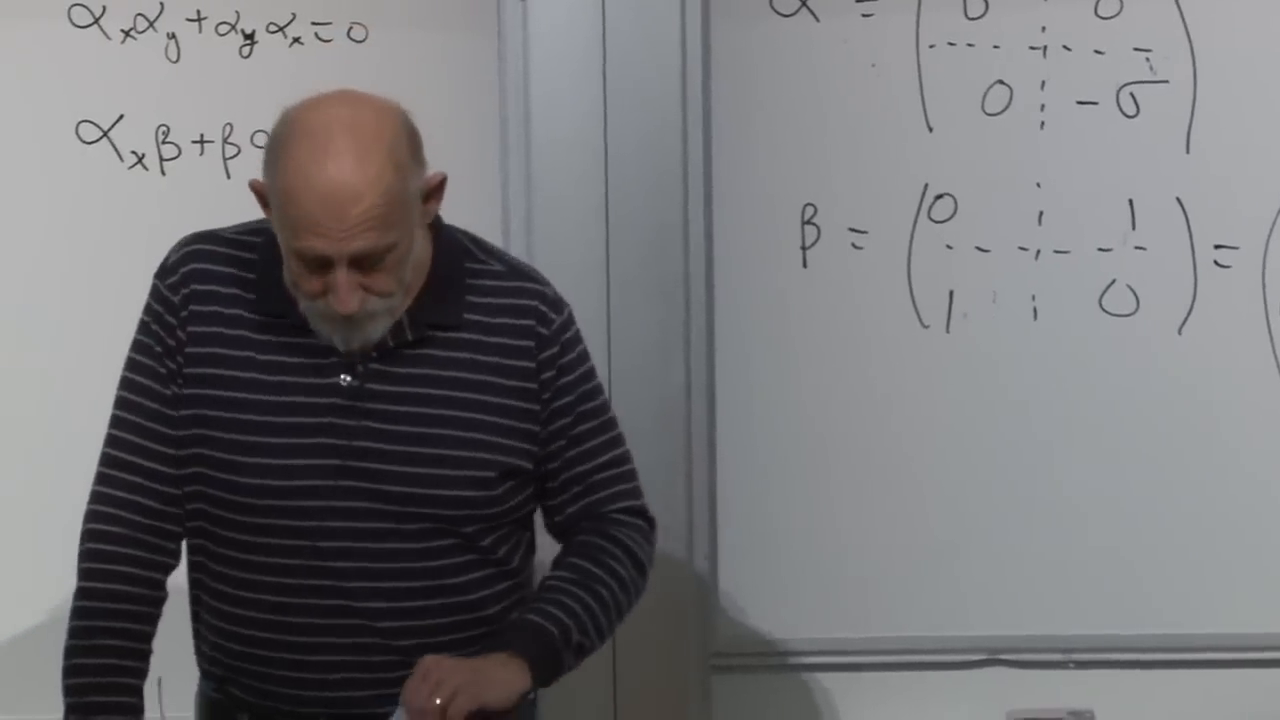
\includegraphics[width=0.94\linewidth]{lecture_10_figure_06.png}
\caption{黒板の\(4\times4\)ブロック表現。上の式は要求される反可換子を記録している。完全な行列は式~\eqref{eq:l10-block-representation}に組版されている。}
\lectureframe{00:41:10}
\end{figure}

質量をもつハミルトニアンは今や
\begin{equation}
H=\boldsymbol{\alpha}\cdot\mathbf P+\beta m
=
\begin{pmatrix}
\boldsymbol{\sigma}\cdot\mathbf P&mI_2\\
mI_2&-\boldsymbol{\sigma}\cdot\mathbf P
\end{pmatrix}.
\label{eq:l10-massive-dirac}
\end{equation}
である。式~\eqref{eq:l10-dirac-algebra}を用いると、
\begin{equation}
H^2=\mathbf P^2+m^2.
\end{equation}
したがって四次元構造は任意の装飾ではない。三次元運動量と質量項の両方を許しつつ方程式を一階に保つ最小の構造なのである。

\section{カイラリティと余分な成分の意味}

この拡大はどのような物理的区別を加えたのか？ まず質量のない上ブロック
\begin{equation}
H_R=\boldsymbol{\sigma}\cdot\mathbf P,
\end{equation}
と、質量のない下ブロック
\begin{equation}
H_L=-\boldsymbol{\sigma}\cdot\mathbf P.
\end{equation}
から始める。正エネルギーの状態について、第一のものはスピンが運動量と整列し、第二のものはスピンが反整列している。これらは反対のヘリシティである。質量のない理論では、ヘリシティは固有ローレンツ変換の下で不変である。なぜなら、いかなる観測者も光速的な粒子を追い越し、そのスピンを変えずに運動量を反転させることはできないからである。したがって二つのブロックは反対のカイラルセクターを記述する。

\begin{classroomqa}
\lecturetimestamp{00:41:28}
\audiencequestion{一次元では質量を導入するために余分な二値的自由度が必要であった。三次元における対応する物理的区別は何か？}
\lecturerresponse{それはスピノルの巻き性である。二つの\(2\times2\)ブロックはスピンと運動量の間の反対の関係を担う。一方は右手型であり、他方は左手型である。\(4\times4\)理論は両方を含む。}
\end{classroomqa}

式~\eqref{eq:l10-massive-dirac}の質量項は非対角的である。それは上ブロックの振幅を下ブロックへ送り、その逆も同様である：
\begin{equation}
\beta m
\begin{pmatrix}
\Psi_R\\
\Psi_L
\end{pmatrix}
=
m
\begin{pmatrix}
\Psi_L\\
\Psi_R
\end{pmatrix}.
\end{equation}
したがって質量は反対のカイラリティ間の結合である。

\begin{classroomqa}
\lecturetimestamp{00:43:58}
\audiencequestion{質量のない粒子はカイラリティを変えられるか？}
\lecturerresponse{ここに示された自由な質量のないハミルトニアンでは変えられない。二つのブロックは分離しているので、右手型または左手型として始まった状態はそのままである。非対角な質量項こそが、\(m\ne0\)のときにそれらを混合するものである。}
\end{classroomqa}

この言葉遣いはブロック表現に対しては正確であるが、粒子が二つの矢印の間で機械的に反転するというイメージはあまり押し進めるべきではない。物理的な主張は波動方程式における行列の結合である。

\begin{classroomqa}
\lecturetimestamp{00:44:50}
\audiencequestion{これらの行列は四元数に組み込まれているのか？}
\lecturerresponse{パウリ行列は四元数単位と密接に関係している。行列\(-i\sigma_i\)は二乗すると\(-\mathbb{1}\)となり、向きの規約を除いて四元数のパターンで乗算される。完全なディラック行列はより大きなクリフォード代数を必要とし、四元数との関連は以下の議論には必要ない。}
\end{classroomqa}

\begin{classroomqa}
\lecturetimestamp{00:46:34}
\audiencequestion{スピンが角運動量であるなら、ここでそれに関連する別個のエネルギー項は存在するのか。}
\lecturerresponse{独立な自由粒子項は加えられていない。スピノル構造はすでに行列を通じて運動項のハミルトニアンに入っている。スピンを外部磁場に結合させれば追加の相互作用項が導入されるが、それは別の問題である。}
\end{classroomqa}

\section{アルファ行列は速度であり、スピンではない}

各\(\alpha_i\)は二つの\(+1\)固有値と二つの\(-1\)固有値をもつ。異なる成分は可換でないため、それらすべてを同時に鋭く測定することはできない。ある成分が何を表すかを同定するには、ハイゼンベルク方程式を用いる。陽に時間依存しない演算子\(L\)に対して、
\begin{equation}
\dot L=i[H,L].
\label{eq:l10-heisenberg}
\end{equation}
ここでは符号の規約はSchr\"odinger発展\(e^{-iHt}\)によって固定されている。

式~\eqref{eq:l10-heisenberg}を位置演算子\(x\)に適用する。行列はスピノル添字に作用し、位置と可換である。一方、\(P_x\)だけが\(x\)と可換でない：
\begin{align}
\dot x
&=i[\boldsymbol{\alpha}\cdot\mathbf P+\beta m,x]\\
&=i\alpha_x[P_x,x]\\
&=\alpha_x,
\label{eq:l10-velocity}
\end{align}
なぜなら\([P_x,x]=-i\)だからである。したがって\(\alpha_x\)は速度演算子の\(x\)成分であり、同様に、
\begin{equation}
\dot{\mathbf x}=\boldsymbol{\alpha}.
\end{equation}

\begin{classroomqa}
\lecturetimestamp{00:51:50}
\audiencequestion{速度成分の測定は本当に\(+1\)か\(-1\)しか与えないのか。}
\lecturerresponse{はい、単位\(c=1\)での瞬時演算子\(\alpha_i\)についてはそうである。一般の状態は固有状態である必要はないので、その期待値はそれらの値の間のどこにでもあり得る。滑らかに輸送される波束は、粒子が質量をもつとき、光速未満の平均速度をもつ。}
\end{classroomqa}

速度は保存されない：
\begin{equation}
\dot\alpha_x=i[H,\alpha_x]\ne0.
\end{equation}
\(\alpha_y\)、\(\alpha_z\)、\(\beta\)を含む項は\(\alpha_x\)と可換でない。したがって、正エネルギー成分と負エネルギー成分の両方を含む状態は、その位置に急速な振動的寄与を示す。これが\emph{ツィッターベヴェーグング}、文字通り震える運動である。

急速な振動に比べて長い時間で平均した後、期待される相対論的速度は
\begin{equation}
\overline{\mathbf v}=\frac{\mathbf p}{E},
\end{equation}
であり、遅い電子に対して\(\mathbf p/m\)に帰着する。

\begin{classroomqa}
\lecturetimestamp{00:54:40}
\audiencequestion{外力なしで自由電子が震えることはニュートンの法則に反しないのか。}
\lecturerresponse{反しない。並進不変性は運動量を保存するので、\(\dot{\mathbf P}=0\)である。ディラック速度演算子は単に\(\mathbf P/m\)ではなく、その急速な振動部分は運動量が固定されたままで変化し得る。時間平均された運動は期待される自由粒子の関係に従う。}
\end{classroomqa}

\begin{classroomqa}
\lecturetimestamp{00:55:22}
\audiencequestion{速度は常に\(c\)なのか。}
\lecturerresponse{一つの\(\alpha_i\)の瞬時測定は固有値\(\pm c\)をもつが、質量をもつ波束は一般に重ね合わせであり、光速未満の期待値をもつ。その平均群速度は\(\mathbf p/E\)である。}
\end{classroomqa}

\begin{classroomqa}
\lecturetimestamp{00:55:30}
\audiencequestion{振動は質量が速度を変化させるものとして描けるのか。}
\lecturerresponse{いいえ。質量は固定されたパラメータである。振動は非可換な速度演算子とハミルトニアン演算子から、あるいは同等にエネルギー部門間の干渉から生じるのであり、変動する質量からではない。}
\end{classroomqa}

\begin{classroomqa}
\lecturetimestamp{00:56:22}
\audiencequestion{瞬時測定が、平均運動が別の向きを指しているにもかかわらず、速度がある向きを指していると見出すことはあり得るか。}
\lecturerresponse{はい。成分演算子は二つの鋭い固有値をもつ一方、繰り返し測定または時間平均測定はより滑らかなドリフトを回復する。}
\end{classroomqa}

スピンという語も注意深く用いなければならない。\(\alpha_i\)は速度の成分、すなわち通常のベクトルとして変換する。この表現における真のスピン演算子は
\begin{equation}
\mathbf S=\frac12\boldsymbol{\Sigma},
\qquad
\Sigma_i=
\begin{pmatrix}
\sigma_i&0\\
0&\sigma_i
\end{pmatrix}.
\label{eq:l10-spin-operator}
\end{equation}
であり、\(\alpha_i\)とは下のブロックの符号だけが異なる。行列は密接に関係しているが、速度とスピンは同じオブザーバブルではない。

\section{負エネルギーと最低エネルギー真空}

負エネルギーの問題は、このような行列の仕組みの前にすでに存在している。一次元の右向き運動に戻ると、
\begin{equation}
H=P.
\end{equation}
\(p\)は実数直線全体を動くので、\(E=p\)には下界がない。

真空は単に粒子が存在しない状態を意味することはできない。それ以上エネルギーを奪えない状態でなければならない。もし空の状態が負エネルギーの粒子を加えることを許し、エネルギーを下げ、さらに別の粒子を加え、以下無限に続けられるならば、その空の状態は安定な真空ではない。

フェルミ統計が歴史的な解決策を与える。すべての負エネルギー状態に電子を1個ずつ置く。電子を追加するたびに全エネルギーは下がるが、排他律により各一粒子状態には電子を1個しか入れられない。すべての負エネルギー状態が埋まると、それ以上電子はこのセクターへ落ち込めない。ディラックはこの埋まった配置を真空と同定した。

同じ構成はボソンでは破綻する。任意個のボソンが1つの状態を占めうるので、負エネルギーのボソン的モードは際限なく粒子を吸収できてしまう。講義の冒頭で導入したフェルミオン的束縛 \(n=0,1\) こそが、この下降を止めるものである。

\begin{figure}[htbp]
\centering
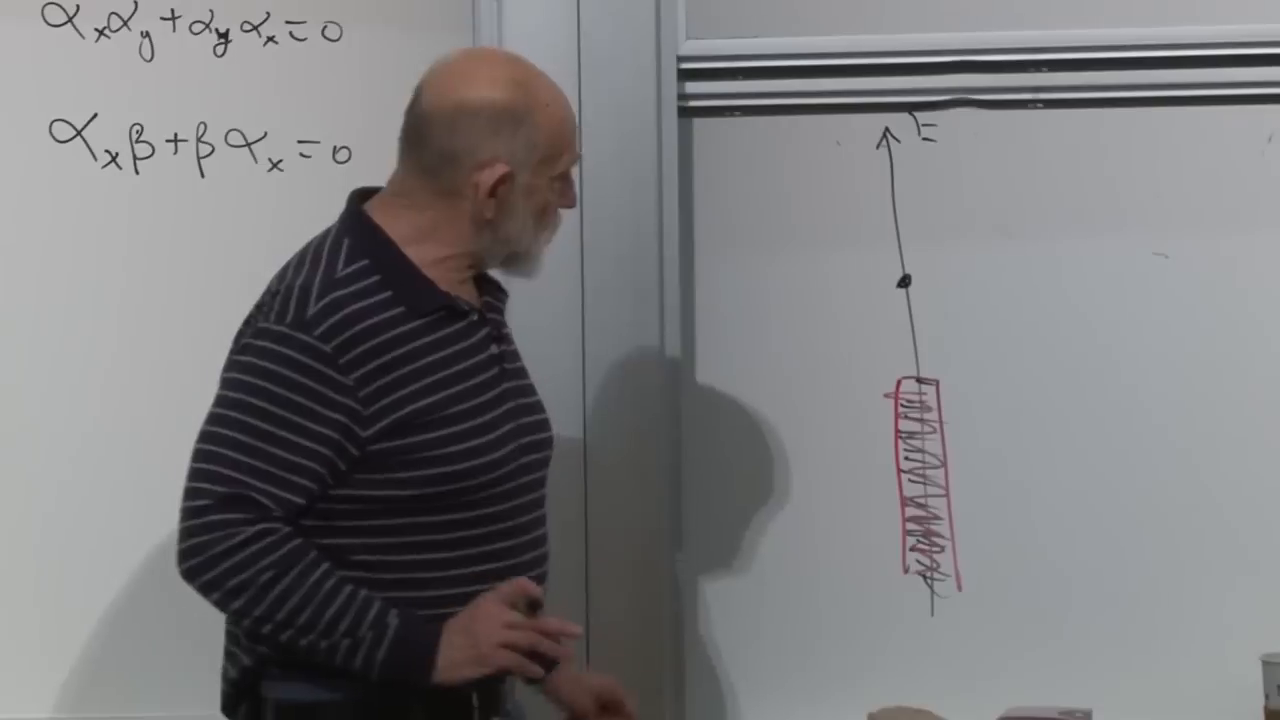
\includegraphics[width=0.94\linewidth]{lecture_10_figure_07.png}
\caption{黒板上の歴史的なディラックの海の描像：負エネルギー準位のはしごが分割線まで埋まり、その上に正エネルギー状態がある。}
\lectureframe{01:02:45}
\end{figure}

\begin{figure}[htbp]
\centering
\begin{adjustbox}{max width=\linewidth}
\begin{tikzpicture}[x=1.05cm,y=0.72cm,>=Latex]
\draw[->] (0,-4.8) -- (0,4.8) node[above] {$E$};
\draw[thick] (-2.9,0) -- (3.2,0) node[right] {$E=0$};
\foreach \y in {-4,-3.3,...,-0.5} {
  \draw (-2.3,\y) -- (2.3,\y);
  \foreach \x in {-1.8,-1.2,...,1.8} {
    \fill[blue!65!black] (\x,\y) circle (1.6pt);
  }
}
\foreach \y in {0.8,1.6,...,4.0} {
  \draw (-2.3,\y) -- (2.3,\y);
}
\draw[red,very thick] (0.6,-2.6) circle (5pt);
\draw[red,->,very thick] (0.6,-2.35) .. controls (1.4,-0.4) and (1.2,1.6) .. (1.5,2.4);
\fill[red] (1.5,2.4) circle (2.5pt);
\node[right,red] at (0.85,-2.6) {hole};
\node[right,red] at (1.7,2.4) {$e^-$};
\node[left] at (-2.5,-2.2) {filled negative-energy states};
\end{tikzpicture}
\end{adjustbox}
\caption{埋まった海の上の励起の明快な再構成：負エネルギーの電子を1個励起すると、正エネルギーの正孔が残る。}
\end{figure}

海の描像は、正しい演算子の再配列に対する歴史的な言葉である。その文字通りの無限の電荷とエネルギーを直接観測可能な量と誤解してはならない。現代的な再定式化は、物質的な電子が空間を満たすと想像する必要を取り除く。

\section{正孔は陽電子である}

すべての負エネルギー状態が占有されているとき、2種類の励起が可能である。海の上に正エネルギーの電子を加えてもよい。あるいは負エネルギーの電子を1個取り除いて正孔を残してもよい。

正孔は、失われた電子とは反対の電荷をもつ。電荷 \(-e\) を取り除くと電荷は \(+e\) だけ変化する。また正の励起エネルギーをもつ。取り除かれた電子が \(E_-<0\) であったなら、埋まった真空を基準に測ったエネルギーは次だけ変化する
\begin{equation}
E_{\mathrm{hole}}=-E_->0.
\end{equation}
正孔は正エネルギーで正電荷の励起、すなわち陽電子である。

光子は海の電子を正エネルギー状態へ励起できる。真空を基準にすると、最終状態は電子と陽電子を含む。時間順序図では、電子については電子数の流れを上向きに描き、陽電子の線は逆向きの矢印で描くのが慣例である。矢印はフェルミオン数または電荷の流れを追うものであり、古典的な小さな速度ベクトルではない。

\begin{classroomqa}
\lecturetimestamp{01:05:14}
\audiencequestion{この描像は電子と陽電子の数が等しいことを要求するか。}
\lecturerresponse{任意の状態については要求しない。真空から出発して中性の対を生成すれば1個ずつ得られるが、状態はすでに過剰な電子または過剰な陽電子を含んでいてもよい。電荷保存は反応を制約するが、すべての許された状態が等しい個数をもつことを要求するものではない。}
\end{classroomqa}

ディラックは当初、正孔が質量において電子と同一で、電荷およびその他の加法的量子数のみが反対の粒子になることを知らなかった。方程式と正孔の構成が、陽電子がよく知られた粒子目録に組み込まれる前に、その予言へと導いた。

\section{1つのフェルミオン場が電子と陽電子を含む}

場の演算子は、歴史的な描像を現代的な代数へと持ち込む。ここではスピノル指数、規格化因子、時間依存性をしばらく抑制する。一次元の場は模式的に次のように展開できる：
\begin{equation}
\psi(x)
\sim
\int_{-\infty}^{\infty}dp\,a(p)e^{ipx}.
\label{eq:l10-full-field-integral}
\end{equation}
右向きの分散関係 \(E=p\) に対して、正の \(p\) は正エネルギーを、負の \(p\) は負エネルギーを表す。積分を分割する：
\begin{equation}
\psi(x)
\sim
\int_0^\infty dp\,a(p)e^{ipx}
+
\int_{-\infty}^0 dp\,a(p)e^{ipx}.
\end{equation}
第二項で \(p=-q\) と置き、\(q>0\) として、満たされた負エネルギー電子の消滅を陽電子の生成として再解釈する：
\begin{equation}
b^\dagger(q):=a(-q).
\end{equation}
すると
\begin{equation}
\psi(x)
\sim
\int_0^\infty dp\,
\left[
a(p)e^{ipx}
+
b^\dagger(p)e^{-ipx}
\right].
\label{eq:l10-electron-positron-split}
\end{equation}
平面波の位相の正確な符号は時空の規約に依存する。不変な内容は、\(\psi\) が電子の消滅演算子と陽電子の生成演算子を含むということである。

\begin{figure}[htbp]
\centering
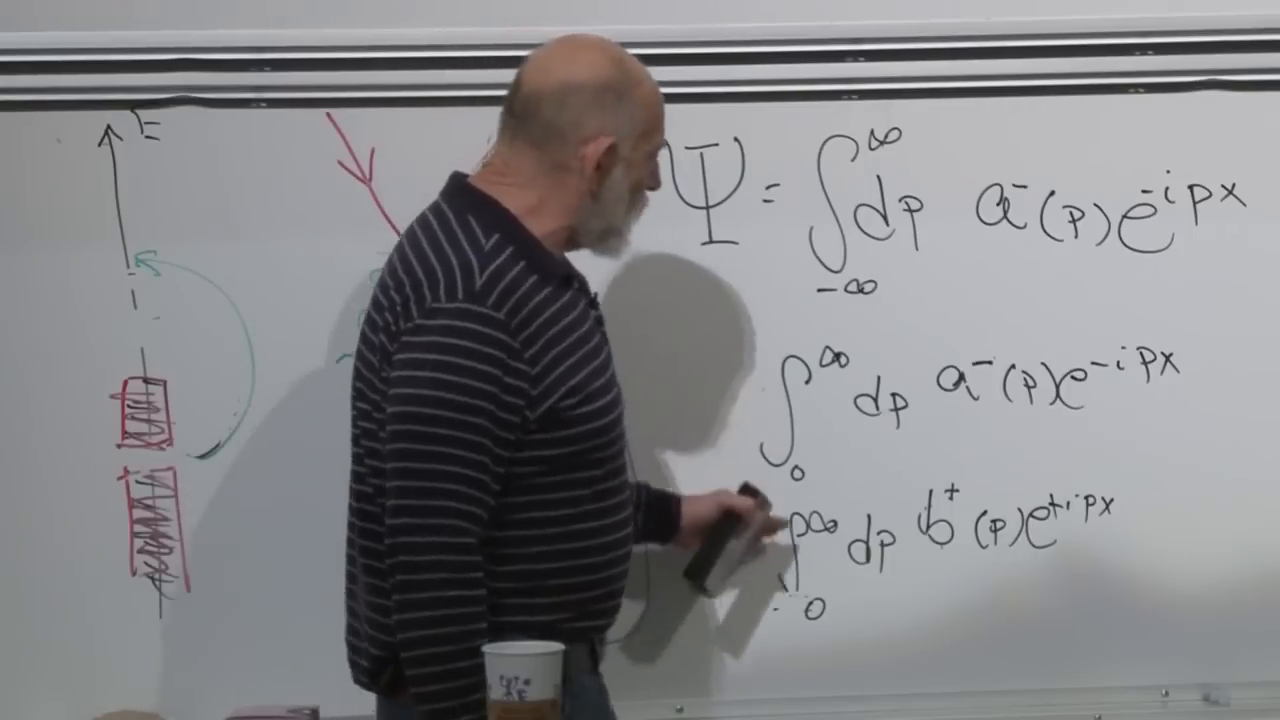
\includegraphics[width=0.94\linewidth]{lecture_10_figure_08.png}
\caption{場の積分を正エネルギーと負エネルギーのセクターに分割したもの。下の行は負エネルギーの電子演算子を陽電子生成演算子として付け替える。}
\lectureframe{01:11:35}
\end{figure}

ここで式~\eqref{eq:l10-fermion-mode}の埋まった-空の対称性が効いてくる。フェルミオンでは、演算子代数はその反交換構造を変えずにこの付け替えを許す。

電磁相互作用の模式的な形は
\begin{equation}
H_{\mathrm{int}}
\sim
\int dx\,\psi^\dagger(x)\psi(x)A(x),
\label{eq:l10-qed-schematic}
\end{equation}
である。ここで \(A\) は光子場を表す。各フェルミオン場は電子と陽電子の成分を含むため、単一の局所演算子がいくつかのチャネルを含む：
\begin{align}
e^-&\longrightarrow e^-+\gamma,\\
e^-+e^+&\longrightarrow\gamma,\\
\gamma&\longrightarrow e^-+e^+,
\end{align}
およびそれらの逆過程と交差過程である。どのチャネルが特定の環境で運動学的に可能かは、エネルギー・運動量保存が決める。例えば、真空中の孤立した実光子は、反跳を吸収する別の参加者がいなければ対を生成できない。局所頂点が相互作用に存在していてもである。

\begin{figure}[htbp]
\centering
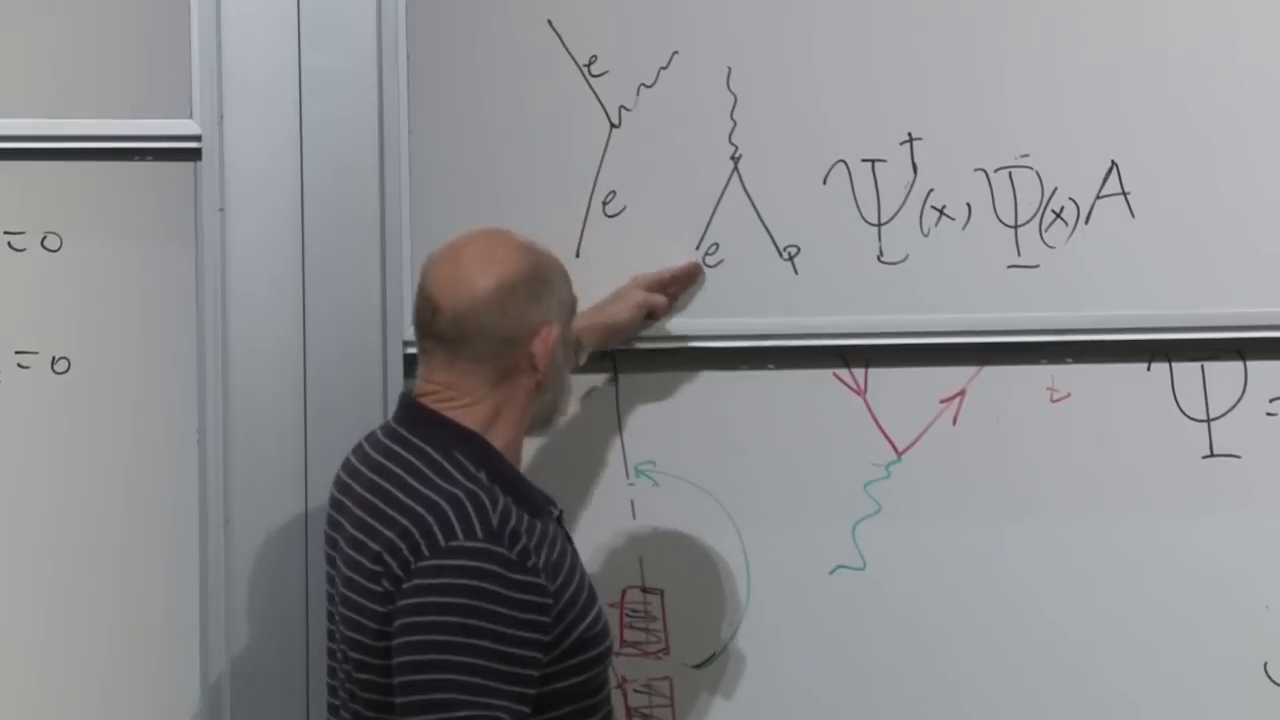
\includegraphics[width=0.94\linewidth]{lecture_10_figure_09.png}
\caption{黒板は電子放出、対消滅、および模式的な相互作用 \(\psi^\dagger\psi A\) を並置している。同じ場の演算子から異なる選択をすることが、異なるチャネルを生み出す。}
\lectureframe{01:13:30}
\end{figure}

したがって、1つのコンパクトな場の積が、多くの見かけ上異なる反応を組織化する。ファインマンは後に振幅を評価するための体系的な図式規則を与えたが、演算子構造の多くはすでにここに見えている。

\section{現代の真空の言語とフェルミ海のアナロジー}

\begin{classroomqa}
\lecturetimestamp{01:14:20}
\audiencequestion{現代の物理学者は、真空を文字通りのディラックの海として扱うことなく、これをどのように記述するのか。}
\lecturerresponse{彼らは演算子の再解釈を直接行う。負エネルギーの電子の消滅は、正エネルギーの陽電子の生成と改名され、真空はすべての電子と陽電子の消滅演算子によって消滅させられる状態として定義される。得られる定式化は粒子と反粒子の間で対称であり、物質的な海を必要としない。}
\end{classroomqa}

歴史的な海は、その論理が凝縮系に近い類似をもつため、依然として有用である。結晶では、固定された数の電子が、フェルミ準位までの利用可能な最低の一粒子状態を満たす。満たされた基底状態は空ではない。1つの電子をその準位より上に励起すると、その下に非占有状態が残る。満たされた背景に対して、正孔は正の励起エネルギーを持ち、正の電荷キャリアとして振る舞うことができる。

重要な違いがある。固体中の正孔は媒質中に存在し、その有効質量と電荷応答はバンド構造に依存する。陽電子は相対論的量子場における素粒子の反粒子である。それでもなお、共通の粒子-正孔代数がこのアナロジーを強力にする。

\begin{classroomqa}
\lecturetimestamp{01:17:14}
\audiencequestion{ボソンに対するKlein--Gordon理論も、負エネルギー状態への同じカスケードに陥るのだろうか。}
\lecturerresponse{いや、そうではない。適切に量子化された複素Klein--Gordon場は、ボソンの海を埋めることなく、正エネルギーの粒子と反粒子へと組織化される。その二階の方程式と正準構造はDiracハミルトニアンの構成とは異なるため、歴史的なフェルミオン的海の議論がそのまま移されるわけではない。}
\end{classroomqa}

\begin{classroomqa}
\lecturetimestamp{01:17:30}
\audiencequestion{ボソンのスピン1はどこから来るのか。}
\lecturerresponse{ここで用いられたパウリ行列の線形化からではない。スピン1の場はそれ自身のローレンツ変換則と場の方程式をもつ。現在の導出はディラックフェルミオンのスピノル構造を説明するものであり、可能なすべての粒子スピンを説明するものではない。}
\end{classroomqa}

\begin{classroomqa}
\lecturetimestamp{01:17:46}
\audiencequestion{なぜフェルミ統計が負エネルギー解に不可欠だったのか。}
\lecturerresponse{排他律が各状態を1つの電子に制限するからである。すべての負エネルギー状態が占有されると、それ以上電子はそれらに落ち込めない。ボソンの占有にはそのような上限がないため、文字通りの負エネルギーのボソンの海には依然として底がない。}
\end{classroomqa}

\begin{classroomqa}
\lecturetimestamp{01:20:02}
\audiencequestion{電子対陽電子は、電荷のように単に別の二値的自由度なのか。}
\lecturerresponse{状態の数え方としては、質量をもつディラック場は2つの電子スピン状態と2つの陽電子スピン状態をもつので、2つの二値ラベルは有用な記憶法である。しかし粒子対反粒子は、1つの電子の独立に回転できる内部量子ビットではない。すべての電子は電荷 \(-e\) をもち、すべての陽電子は \(+e\) をもち、その区別は量子化後の正周波数と負周波数のセクターから現れる。}
\end{classroomqa}

無限の海は最後に1つの疑問を提起する。

\begin{classroomqa}
\lecturetimestamp{01:20:54}
\audiencequestion{無限のディラックの海は無限の宇宙定数を生み出すのだろうか。}
\lecturerresponse{それは真空エネルギーの問題を露呈させる。ボソンの零点モードは\(+\tfrac12\hbar\omega\)に寄与するが、フェルミオン的モードは逆の符号で寄与する。スペクトルが一致する場合には形式的な相殺が可能であるが、電子と光子のスペクトルは一致せず、莫大な残差が予想される。重力がなければ、エネルギーの差のみが重要であるため、ハミルトニアンの定数シフトは差し引くことができる。重力があれば、絶対的な真空エネルギーが重力に寄与するため、その差し引きは単なる帳尻合わせではなく物理的な問題となる。}
\end{classroomqa}

最後に戻るのは質量の意味についてである。

\begin{classroomqa}
\lecturetimestamp{01:22:56}
\audiencequestion{質量が左手系成分と右手系成分をどのように関係づけるかについて、さらに言えることはあるだろうか。}
\lecturerresponse{正確な記述はすでにハミルトニアンの中にある。非対角項\(m\beta\)が一方のカイラルブロックを他方へ写すのである。微視的な反転についてこれ以上に力学的な描像を与えることは任意であり、必然的に不完全である。}
\end{classroomqa}